\documentclass[twoside,10pt]{article}
\setcounter{secnumdepth}{5}
\usepackage{amsmath,amsfonts,amsthm,fullpage}
\usepackage{algorithm}
\usepackage{algorithmic}
\usepackage{graphicx}
 

\begin{document}

\title{Report - Special Problem }
\author{Dr. Bistra Dilkina , Parminder Bhatia}
\date{}
\maketitle

%----------------------------------------------------------------------------------
\section{Introduction}
Spatial Optimization is one of the most important problem in computational sustainability today. For the purpose of understanding ,we can consider that if we are given a raster matrix (M*N), spatial optimization can be described as allocation of land types (Commercial, Residential, Green,Industrial, Recreational) to each of the cells /land mass under given constraints (money, contiguity, future expansion etc.).  Spatial Optimization is challenging because it involves lots of dependencies, variables, objectives and input parameters. And as these features increase the problems becomes more complex and it grows exponentially. Solving such a massive problem manually is out of question. We need computational tools to better understand all the aspects of such a gigantic problem.
Comprehensive sustainability in urban planning can be termed as a long-term balance between economic development, environmental protection, efficient resource use, and social equity


Spatial Optimization can also be looked as a demand-constraint problem, where objective is to allocate land type of given land masses keeping in mind the various constraints. The abstract concept of constraints on which  desired constraints and objectives are build are :-
Continuity
Compactness
Compatibility

\graphicspath{ {images/} }
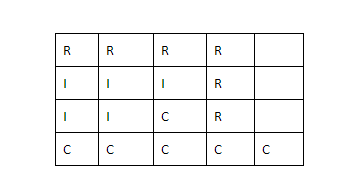
\includegraphics{raster}

\subsubsection*{Continuity} - Continuity can be defined as as the degree to which a specific use has been allocated to land in an unbroken fashion. It basically refers to the connected component of the same type. Here, in the figure we can see that C has very high contiguity.

\subsubsection*{Compactness} - We define compactness as an allocation of a given land use to sites that are in direct proximity of each other, resulting in circular patches. In the figure above, we can see that land type I has maximum compactness.

\subsubsection*{Compatibility} - Compatibility  as the word suggests refers to how compatible a given land use type is with his neighbour(other land type) . We would prefer to have green areas close to residential as compared to having industry close to residential, thus compatibility index of the former will be higher.\\[.25cm]

In a land usage optimization problem, finite amount of resources (commercial, industrial, residential area etc.) are allocated effectively to a specific land mass under given constraints (money, contiguity, future expansion etc.). In fact it has been depicted that inefficient resource use leads to high traffic congestion and other sustainability issues (Newman et al.). Therefore, it is important to carefully design land use allocation models. Since, land use allocation is a resource allocation problem for a given space, therefore many times it is considered as a spatial optimization problem. \\
This problem was first addressed by Schlager et al. as a Linear Programming model in 1965 and it was mostly constrained to single objective optimization. Since this problem is much more complex and involves a lot more objectives, therefore multi-objective approach was adopted by other researchers (mentioned in following section).  Many researchers however constrained themselves by still continuing with Linear Programming approach and by assigning different weights to different objectives and performing linear combinations to attain the solution.It is a major issue for planners to numerically quantify the relative weights of each of the defined objective. Moreover, non-convex optimal solutions cannot be obtained by minimizing linear combinations of objectives.


Due to the multifaceted nature of land-use allocation, spatial optimization modelling should aim at finding a set of high-performing alternatives instead of just one solution (Bankes 1993, Church 1999, Harris 2001) and allow the stakeholders to choose from a number of scenarios that are both good and different from each other, since not every planning objective of interest may be introduced into the
model in the form of mathematical formulation (Chang et al. 1983, Brill et al. 1990). The decision-makers should be provided with alternatives that allow for consideration of other—less defined—planning goals, or recognition of overlooked issues and innovative solutions (Chang et al. 1983). Consequently, the generated alternatives should be treated not as ultimate solutions but as propositions for further analysis by stakeholders.
\section{Summary of earlier work}

\subsubsection{Multi Objective Land Use Problem -Zielinska}

\paragraph*{Minimize Development of open space} Consider values Aj  for all cells that encode attractiveness for development for undeveloped cells. Idea is to set Aj very low for cells in open space. Add objective to minimise summation of (1-Aj) for all undeveloped cells that are developed. 
\paragraph*{Minimize redevelopment of urban areas}  Here idea is to avoid redevelopment of already developed areas . Here we define variable Rj as resistance for cell j to change from one developed form to another. This value will be high for compatible and contiguous neighbours and can be set low for cells which have low compatibility with his neighbours.
\paragraph*{Minimize incompatibilities between land use of site j and its neighbourhood } Here, there are 2 scenarios. First when an undeveloped cell is developed to type j. We want to minimize its compatibilities with its dominant neighbours. Thus , we would like to maximize developing cells with high compatibility. Second case is for  cells which are already developed and are changed from type i to j. Similar to previous premise , we want  to minimize its compatibilities with its dominant neighbours. 
\paragraph*{Minimizes the distance of new development to already developed sites } In order to increase compactness and avoid scattered developed areas , we want that newly developed areas should be in close proximity to the already developed areas.
\paragraph*{DBDC}
This step is important as it represents a contiguity and compactness constraint,which forces a user-specified neighbourhood infill development . It ensures that we will allocate to cell j if and only if the sum of the j?s initially and newly developed neighbours is at least equal to threshold b.\\[.25cm]


\subsubsection{Spatial multi-objective land use optimization: extensions to the  non- dominated sorting genetic algorithm-II -CAO}
\paragraph*{Minimizing land conversion costs}
Here it simply converts the minimization of conversion costs to the minimization of land use changes which clearly leads to greater economic benefits. However, this may rather lead towards to change from existing .

\paragraph*{Maximizing spatial accessibility}
Accessibility is important for land use planning not only because it reflects the operational efficiency of a city, but also because good accessibility planning can also improve social equity and lead to decreases in CO2 and related emissions which are largely generated inside the city from various human and automobile activities . The road system can be divided into three types:
roads that primarily serve residential neighborhoods, major routes for all transportation,
and routes that serve commercial and mixed uses.

Accessibility can be defined as how close or in proximity we have a Road of type R to location E[i,j].

Increasing land use compatibilities \\[.15cm]

The NSGA-II-MOLU model \\
Chromosome - Chromosome representation is a list or grid of genes, where the position of each
gene (cell) represents a unit and the land use of the unit is determined by its value.


\subsubsection*{Operators for NSGA-II-MOLU}
Paper on Cao was crucial from the perspective of defining operators to be used for NSGA II . \\
\paragraph*{Initialization operators}
In land use optimization problems, data pertaining to the existing land use status quo should be used as part of the iteration process, and then the initialization operators will create 90% random solutions and 10% land use status quo solutions as part of the initialized population. This initialization operator is called the problem-based initialization operator (PBIO).
\paragraph*{The crossover operator}
The crossover usually operates between the parents that are the two chromosomes from the population. However, in terms of the characteristics of the solution, self-reproduction might be made more efficient for each chromosome. The single parent crossover operator (XSP), which represents the two-dimensional structure of the spatial landscape, is applied to the land use optimization based on NSGA-II.

\paragraph*{Mutation operators}
There are two mutation operators. First operator(MPC) maintains diversity among solutions in a population, and the second is the mutation by constraint steering (MCS) which erases infeasible solutions from the population and enables the constraints to be met. 

\subsubsection{Evolutionary Multi-objective Optimization for landscape system design - Roberts}
 Based on Natural Habitats optimization . It uses methodology for generating estimates of the Pareto optimal set of designs for an evolving landscape in the rural urban fringe of a major metropolitan area.\\
 General landscape ecological principles
\begin{itemize}
  \item Patch size The term patch refers to a contiguous extent of natural features across
a landscape. In general, larger patches are better than smaller patches for
sustaining natural ecological functions.
  \item Number of patches Reducing the number of patches across a landscape reduces
the potential for recolonization and the potential for biodiversity by reducing the
availability of specific habitat types.
  \item Patch location If small patches are isolated islands then, depending on the
distance they are from other similar habitats, the populations they harbor are at a
greater or lesser risk of extinction.
  \item Patch shape -  Patches which are disc shaped allow for more interior habitat for a
given area and thus the potential for more interior species is increased. Convoluted
edges, i.e., lobes or peninsulas, encourage interactions with surroundings and favor
edge and/or generalist species.
\end{itemize}

\paragraph*{Objectives}
Considering the various features/concepts following are the objectives ,  the following four landscape level configuration patterns are deemed critical.

\begin{itemize}
  \item A few large patches of natural vegetation
 \item  Vegetated major stream or river corridors
 \item   Connectivity between larger patches with natural corridors and stepping stone patch configurations.
 \item  Heterogeneous patches of natural habitat dispersed throughout the landscape.
\end{itemize}
\paragraph*{Objective Functions}
\begin{itemize}
  \item OF1 - rewards maximizing the area of natural vegetation features in the entire data
set using the ELC classes normalized by total area.
 \item OF2 This objective rewards solutions with a few large patches of natural features which may be heterogeneous, e.g., comprising both woodland and wetland features.
 \item OF3 This objective favors connected structures of natural features across the landscape by maximizing the number of connected components in the top 1 to 5 (by area weighted, area?perimeter ratio) natural area subgraphs.
 \item OF4 This objective function rewards the formation of
discontinuous chains of smaller patches as pathways between larger vegetated
patches.
 \item OF5 This objective function rewards maximizing the area of agri/silvicultural features, normalized by total area,

\end{itemize}
\section{Conventions}
Let us first define the conventions we will use for variables . \\ 
\begin{itemize}
\item Landuse : Landuse specifies the type of land allocation to that particular area. They can take values from 0 to N, where N is the number of landuse types. We will always refer to 0 as the undeveloped land type and others would be enumerated depending upon the number of land types available. To refer to particular area we will use the notation $X_{ik}$, where land/pixel i is assigned a landuse type k.
\item Attractiveness : We define $a_j$  as the measure of attractiveness of an undeveloped location for development. 
$ a \in (0,1)$
\item Area : $A_j$ is the area of the parcel j.
\item $Y_i$ is the initial land use type of parcel $i \in V$
\item V : Refers to all the parcels /cells

\item U : Refers to set of parcels that are undeveloped \\
 
$ Y_{i} = 0$ , where  $Y_{i}$ refers to the land use type. 
\item $N_j$ : Neighbours of parcel $j \in V$    
\item Compatibility : $\partial_{kk'}$ refers to compatibility of landuse type k with k', where k,k' $\in {0,..N}$
\item : Closest Neighbour -  $dist_j$ refers to distance from j to closest developed neighbour cell.
\item $\vartheta_{kk'} $ - Refers to the conversion cost from  type k to k'
\item $s_j$ : Number of initially developed neighbours of j , $$ s_j = \sum_{i \in N_j: Y_i \neq 0} 1$$
\item $rd_j$ : road distance to the closest road from cell  j
\item roadDist(dis,k) : It is the penalty for distance from road for type k


\item
\subsubsection*{Minimize Undeveloped Land}

We define $ a_{j},$ as the attractiveness of an undeveloped location for development. Higher value indicates higher attractiveness towards development.  Thus, we can have low value for undeveloped open places. and minimize the following

 $$
 min\sum_{j \in U} (1-a_j) \sum_{k=1}^N X_{jk}
 $$
Consider values $a_j$  for all cells that encode attractiveness for development for undeveloped cells. Idea is to set $a_j$ very low for cells in open space. Add objective to minimise summation of (1-$a_j$) for all undeveloped cells that are developed. 

\item 
\subsubsection*{ Compatibility(special version of contiguity)}
All earlier papers have tried to make use of compatibility by keeping static locations , where they compare compatibility of new allocation with respect to static initial allocation.
 $$
max \sum_{j \in U} \sum_{i \in N_j}(\sum_{k=0}^{N}\partial_{kk'} X_{jk} X_{ik'})
 +max \sum_{j \in V} \sum_{i \in N_j}(\sum_{k=0}^{N}\partial_{kk'} X_{jk} X_{ik'})
 $$
 This basically means , that we assume neighbors to be same(static across the selection) 

We would like to maximize compatibility of a cell wrt its neighbours.
$$
max \sum_{j \in V}  \sum_{i \in N_j}(\sum_{k=0}^{N}\sum_{k'=0}^{N}\partial_{kk'} X_{jk} X_{ik'})
 $$
Here $N_j $ are neighbours of j. Thus we want development such that compatibility is maximised. Simple equivalent of this would be to have $\partial_{kk'} = 1 $ if  $k =k'$ else $0$

\item
\subsubsection*{ New Development}
Next objective is to keep new developments close to existing developments
 $$
 min\sum_{j \in U}(dist_j) \sum_{k=1}^N X_{jk}
 $$

\item

\subsubsection*{Minimize land conversion }
Minimize land conversion -- Conversion cost refers to the cost associated with changing the landuse type of parcel from one type to another.
$$
 min\sum_{j \in V}  \sum_{k=1}^N (\vartheta_{Y_{j}k}) X_{jk}
 $$
In the simple version, we can keep $\vartheta_{Y_{j}k} =  1$ for all k where $k \neq Y_{j},0$
\item
\subsubsection*{Compact Development -- Infill development}
All earlier papers have tried to make use by keeping static locations , where they compare compact development of new allocation with respect to static initial allocation.
Idea is that if j is developed then atleast b of his neighbours should be developed.
$$
s_j +\sum_{i \in N_j, Y_{i} =0 } \sum_{k"=0}^N X_{ik"} >= b \sum_{k=0}^N X_{jk}
 $$
\item
\subsubsection*{Accesibility  }
Idea is that particular development should be close to road for accessiility purposes. We are keeping it simple assuming only a single type of road, which can be extended further.
 $$
 min\sum_{j \in V} \sum_{k=0}^N roadDist(rd_j,k)X_{jk}
 $$

\item
\subsubsection*{Assignment Constraint}
$$\sum_{k=0}^N A_j X_{jk} =1$$

\item
\subsubsection*{Demand Constraint  }
 Total area for each type should remain in the upper and lower bound of the limits provided.
$$ L_k < \sum_{j \in V} \sum_{k=0}^N X_{jk} < U_k $$
\end{itemize}


\section{Raster Data}
\subsubsection*{Approach }

With view to validate the Objectives and Constraints defined above, we have implemented the above objectives and we used a synthetic 10 by 10 Raster to observe the impact  of these objectives and constraints.\\[.25cm]

We have implemented the following Objectives:

\paragraph*{Compatibility}

We implemented the special version of contiguity for this objective, where we give weight of 1 to $\lambda_{ij}$ if i and j are same and 0 otherwise.
We  take the continuity objective as a dynamic constraint, where we take the fitness score wrt to current assignment of the candidate. 

\paragraph*{Limits}

We implemented the Limits constraint as an  objective, where we try to minimize this objective. High penalty is given incase the objective does not lie the limits and max negative value is given for land type in the middle of max-min allowed for the above lands type. 

\paragraph*{Attractive}

We implemented the Attractiveness  objective, where we try to minimize this objective. This objective basically suggests that more the attractive of unused land type higher are the chances of it getting developed.

\paragraph*{Conversion}

We implemented the Conversion  objective, where we try to minimize this objective.Minimize land conversion -- Conversion cost refers to the cost associated with changing the Land use type of parcel from one type to another.

\subsubsection*{Implementation Specifics Note}

In the mutation and initial generation for NSGA, we have made sure that each parcel gets value from the allowed lands type for the particular parcel, which makes sure that we don't generate any infeasible solution.
\section{Results and Implementation }
\subsection{Implementation}
In order to validate our objectives, we first analysed our algorithm on a small dataset represented by 10X10  , as shown in the figure.
\begin{figure}[h]
\begin{center}
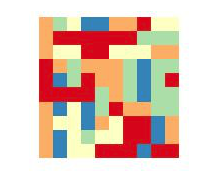
\includegraphics[width=3.in]{orig.png}
\caption{Synthetic Dataset used for initial evaluation}
\end{center}
\end{figure}
In this raster we have 5 types of the LandUse types - Undeveloped, Green, Residential,Commercial and Industrial. 
Here the red region corresponds to undeveloped region.\\
In our implementation, we evaluated and implemented the following objectives. 
\begin{itemize}
\item \textbf{Contiguity} - We evaluated the contiguity by checking for the neighbors which have same assignment of LandUse type as the LandUse type of a particular parcel. We evaluated the neighbors Landuse type based  on the dynamic / current assignment of the candidate.
\item \textbf{Attractiveness} - Attractiveness(a) is defined as willingness of a cell/parcel towards development. We evaluate (1-a) , thus this value will be initially 0 and increase as we change undeveloped cells to developed. Our objective is to minimize this value, thus cells having high attractiveness value will be developed in preference to others.
\item \textbf{Limit} - We want all land use type to be within the min-max limit allocated for the landuse type. We have taken couple of approaches in this. Simple one is to simple give 0 weight when within the limit and apply penalty equal to the extent with which lands is above or below the limit( linear) .Second approach is that instead of simply keeping 0 we made a linear triangle with in the limit which was maximum at center of max-min and give higher penalty when out of range. Note that using this approach gives us a higher bound and more penalty incase of getting out of limits. 
\item \textbf{Conversion} - It is the cost associated with changing lands type from one type to another. \\
\end{itemize}
\subsubsection{NSGA}
\textbf{Generator}- Initially , we generate a sample of dataset. They are generated based on initial configuration and set of allowed changes for some of the parcels. \\[.15cm]
\textbf{Evaluator }- In the evaluator , we basically evaluate the  given candidates based on the objective functions and sign score to each candidate.\\
Based on these scores next generation candidates are selected from the given candidates . \\ [.15cm]
\textbf{Mutation }- In the mutation and initial generation for NSGA, we have made sure that each parcel gets value from the allowed lands type for the particular parcel, which makes sure that we don't generate any infeasible solution.\\[.35cm]

\subsection{Results}
In the current approach we convert all the constraints also into objectives. So , now limits  for Landuse types would also come under the Objective function . We will later use constraint changed objectives only for filtering the results. So , our final output would consist of only results which follow the limit constraints.
We applied the algorithm  on the raster using the following objective functions. \\
\begin{itemize}
\item Contiguity
\item Attractiveness
\item Limit
\end{itemize}
Here there are two approaches of using Limits as Objective. We can make Limit as a combined single objective or can have individual objectives corresponding to each LandUse type . \\
We ran the algorithm using the above objectives, where (X axis) we wanted to maximize continuity(compatibility) and wanted to minimize the attraction (Y axis) .\\
Here we can see the impact of taking limits as Single or Multi Objective Solution.
The results show the parent front (blue dots) formed where there is increase in contiguity (compatibility) of resulting solutions. The results are more compatible and still follow the limit constraints.(as can be seen from the continuity score). \\[.25cm]
The figure below shows the evaluation using NSGA. The  Limits are used as Objective, but its only used for filtering. We only consider solutions which fall in the limits. \\
 One point to notice here is that (Figure 3), using limits as single objective gives better results because if we have too many side objectives which we will eventually filter, then it will have an impact on our primary objectives.\\
\begin{figure}[h]
\begin{center}
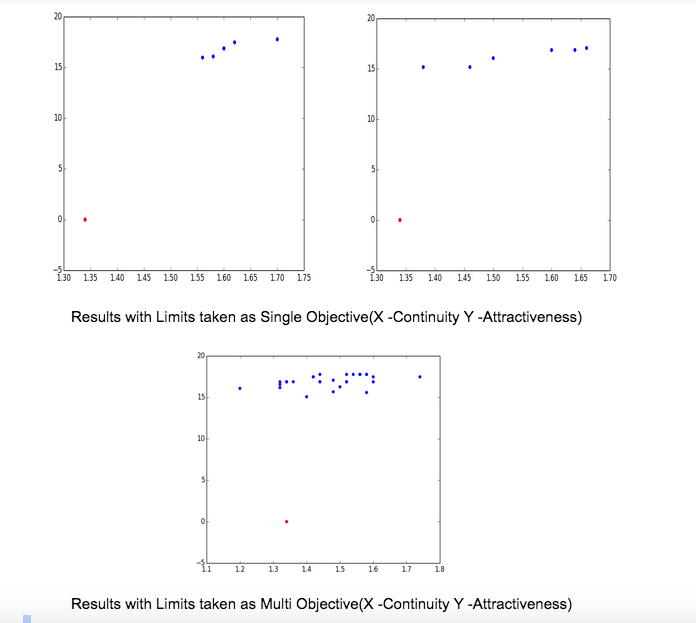
\includegraphics[width=5.in]{comp.png}
\caption{Using Limits as MultiObjective vs Single Objective}
\end{center}
\end{figure}


\begin{figure}[h]
\begin{center}
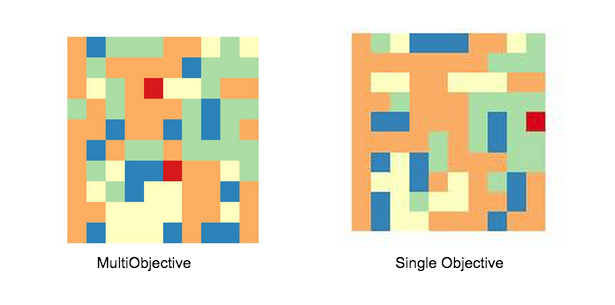
\includegraphics[width=4.in]{mvs.png}
\caption{Using Limits as MultiObjective vs Single Objective}
\end{center}
\end{figure}
\newpage
\section{North Carolina Dataset}
Todo: Results and Impact
We did the similar analysis on North Carolina Dataset
\section{Impact of Dynamic Constraints}
An important difference in our approach is making the constraints dynamic, where the equations we obtained  for compatibility (contiguity) are based on dynamic allocation/constraints keeping in view the present allocation of parcels for a given parents-front /candidate solutions.\\

Following is the plot we obtained for static allocation vs  dynamic allocation. \\

\begin{figure}[h]
\begin{center}
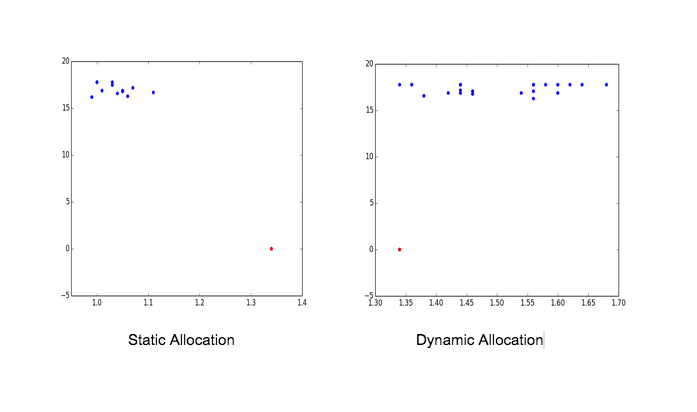
\includegraphics[width=4.in]{svd.png}
\caption{Using Limits as MultiObjective for Static and Dynamic}
\end{center}
\end{figure}
\newpage
\section{Conclusion}
TODO
%\bibliographystyle{plain}
%\bibliography{temp,externalPapers,groupPapers}

\end{document}















